\documentclass[12pt,english]{article}
\usepackage[T1]{fontenc}
\usepackage[latin9]{inputenc}
\usepackage{amsthm}
\usepackage{amssymb}
\usepackage{amsmath}
\usepackage{graphicx}
\usepackage{listings}
\usepackage{color}
\makeatletter
\usepackage[letterpaper,body={6.5in,9in}, head=34pt, foot=70pt]{geometry}
\usepackage{fancyhdr}

\pdfpagewidth 8.5in
\pdfpageheight 11in

\pagestyle{fancy}
\headheight 35pt

\rhead{}
\chead{}
\lhead{}
\renewcommand{\footrulewidth}{0.4pt}
\rfoot{\thepage}
\cfoot{}
\lfoot{}

\definecolor{mygreen}{rgb}{0,0.6,0}
\definecolor{mygray}{rgb}{0.5,0.5,0.5}
\definecolor{mymauve}{rgb}{0.58,0,0.82}
\newcommand{\red}[1]{\textbf{\textcolor{red}{#1}}}


\usepackage{multicol}

\makeatother

\usepackage{babel}
\begin{document}

\lstdefinestyle{mystyle}{ 
  backgroundcolor=\color{white},   % choose the background color; you must add \usepackage{color} or \usepackage{xcolor}; should come as last argument
  basicstyle=\footnotesize,        % the size of the fonts that are used for the code
  breakatwhitespace=false,         % sets if automatic breaks should only happen at whitespace
  breaklines=true,                 % sets automatic line breaking
  captionpos=b,                    % sets the caption-position to bottom
  commentstyle=\color{mygreen},    % comment style
  escapeinside={\%*}{*)},          % if you want to add LaTeX within your code
  extendedchars=true,              % lets you use non-ASCII characters; for 8-bits encodings only, does not work with UTF-8
  firstnumber=1,                   % start line enumeration with line 1
  frame=shadowbox,	               % adds a frame around the code
  keepspaces=true,                 % keeps spaces in text, useful for keeping indentation of code (possibly needs columns=flexible)
  keywordstyle=\color{blue},       % keyword style
  language=MATLAB,                      % the language of the code
  morekeywords={end,to,},          % if you want to add more keywords to the set
  numbers=left,                    % where to put the line-numbers; possible values are (none, left, right)
  numbersep=5pt,                   % how far the line-numbers are from the code
  numberstyle=\tiny\color{mygray}, % the style that is used for the line-numbers
  rulecolor=\color{black},         % if not set, the frame-color may be changed on line-breaks within not-black text (e.g. comments (green here))
  showspaces=false,                % show spaces everywhere adding particular underscores; it overrides 'showstringspaces'
  showstringspaces=false,          % underline spaces within strings only
  showtabs=false,                  % show tabs within strings adding particular underscores
  stepnumber=1,                    % the step between two line-numbers. If it's 1, each line will be numbered
  stringstyle=\color{mymauve},     % string literal style
  tabsize=2,	                   % sets default tabsize to 2 spaces
}

\textbf{}\vspace{0.4cm}

\textbf{Due: } \textbf{}\vspace{0.6cm}

\begin{enumerate}
    \item Consider the following nonlinear programming problem
            \begin{align*}
            \text{minimize}\ \ x_1^2+x_2^2\\
            \text{subject to }\ \ 2x_{1}x_{2} & = 3
            \end{align*}
    Do a \textbf{contour map} of the function $f(x_1,x_2) = x_1^2+x_2^2$ and superimpose the relation given by equality constraint $h(x_1,x_2) = 0$, where $h(x_1,x_2) = 2x_{1}x_{2}-3$ \vskip 2ex
    You can use MATLAB to do this. For example, modify the code below to plot both the level curves of $f$ and $h(x_1,x_2) = 0$\vskip 2ex
\lstset{style=mystyle}
\begin{lstlisting}
[X,Y] = meshgrid(-2.0:.2:2.0,-2.0:.2:2.0);
Z = X.^2+Y.^2;
P = 2.*X.*Y-3;
[c,h]=contour(X,Y,Z);
clabel(c,h);
hold on;
[v,j]=contour(X,Y,P);
clabel(v,j);
grid on;
xlabel('x_1');
ylabel('x_2');
syms X Y Lambda 
F = X^2+Y^2;
H = 2*X*Y-3;
L = F + Lambda * H;
g = gradient(L, [X, Y, Lambda]);
disp(g);
\end{lstlisting}
\begin{center}
    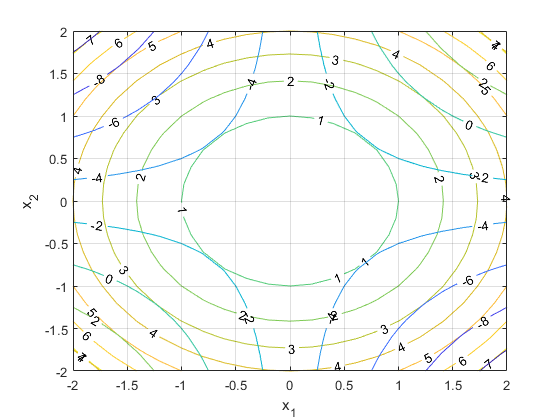
\includegraphics[width = .6\textwidth]{ContourLines2.png}   
\end{center}

\pagebreak
    \begin{enumerate}
        \item Define the Lagrangian function
        \[\mathcal{L}(x_1,x_2,\lambda) = f(x_1,x_2) + \lambda h(x_1,x_2)\]
        \[\boxed{\mathcal{L}(x_1,x_2,\lambda) = x_1^2 + x_2^2 + \lambda(2x_1x_2-3) = x_1^2 + x_2^2 + 2\lambda x_1x_2-3\lambda}\]
        Also defined in line 12.\vskip 2ex
        \item Calculate the \textbf{gradient} of $\mathcal{L}$
        \[\nabla\mathcal{L} = \begin{bmatrix}\frac{\partial \mathcal{L}}{\partial x_1}\\\frac{\partial \mathcal{L}}{\partial x_2} \\ \frac{\partial \mathcal{L}}{\partial \lambda}\end{bmatrix} = \begin{bmatrix}2x_1 + 2x_2\lambda\\2x_2 + 2x_1\lambda\\ 2x_1x_2-3\end{bmatrix}\]  
        \item Find $x_1^\star,x_2^\star$, and $\lambda^\star$ such that
        \[\frac{\partial \mathcal{L}}{\partial x_1} = 0\]
        \[\frac{\partial \mathcal{L}}{\partial x_2} = 0\]
        \[\frac{\partial \mathcal{L}}{\partial \lambda} = 0\]
        and compute the value of $f$ at $(x_1^\star,x_2^\star) $\vskip 2ex
                
        We can rewrite the question as a system of equations. The partial derivatives are calculated above.
        
        \[\begin{array}{rcr}
            2x_1 + 2x_2\lambda & = & 0 \\
            2x_2 + 2x_1\lambda & = & 0\\
            2x_1x_2-3 & = & 0
        \end{array}\]
        Using wolfram to solve gives us four solutions.
        \[\nabla\mathcal{L} = 0 \begin{cases} x_1 = \pm \sqrt{\frac{3}{2}},~x_2 = \pm \sqrt{\frac{3}{2}},~\lambda = -1 \\ x_1 = \pm i\sqrt{\frac{3}{2}},~x_2 = \pm i\sqrt{\frac{3}{2}},~\lambda = 1\end{cases}\]
        Both of the real solutions, when evaluated on the objective function give 3 as a result.
        \item Is the point $(x_1^\star,x_2^\star)$ found in part (c) the \textbf{optimal solution} for problem (1)? Justify your answer.\vskip 2ex
        By definition, the solution corresponding to the original constrained optimization is always a saddle point of the Lagrangian function. The Hessianis test applied on this problem is inconclusive, so I'm not able to confidently say this solution is the best, however my intuition says it is.
       
    \end{enumerate}
    \pagebreak
    \item Consider the function $f: \mathbb{R}^2\rightarrow \mathbb{R}$,
    \[f(x_1,x_2) = 8x_1+12x_2+x_1^2-2x_2^2\]
    \begin{enumerate}
        \item Show that the function $f(x_1,x_2)$ \underline{has only one} \textbf{stationary point} (i.e. a point where $\nabla f(\mathbf{x^\star})=(0,0)$). \vskip 2ex
        
        We can start by completing the requisite partial derivatives \[\frac{\partial f}{\partial x_1} = 2x_1+8 \text{ and } \frac{\partial f}{\partial x_2} = -4x_2+12~~~~~ \therefore \nabla f(\mathbf{x}) = \begin{bmatrix}2x_1+8 \\ -4x_2+12\end{bmatrix}\] 
        Stationary points occur at points where the gradient is zero, so we can just set each expression to zero and solve.
        
        \[2x_1+8 = 0 \rightarrow x_1 = 4\text{ and } -4x_2+12=0 \rightarrow x_2 = -3\]
        This is the only solution to these equations, thus it is also the only stationary point for the equation.
        \vskip 2ex
        \item Show that the stationary point is \underline{neither a maximum nor a minimum}.\vskip 2ex
        
        We can show this by computing the Hessian matrix and using its determinate to conclude the properties of the point. We will start by computing the requisite partial derivatives. \[\frac{\partial^2 f}{\partial x_1^2} = 2,~ \frac{\partial^2 f}{\partial x_1 \partial x_2} = 0,~  \frac{\partial^2 f}{\partial x_2 \partial x_1} = 0,\text{ and } \frac{\partial^2 f}{\partial x_2^2} = -4\]
        Therefore our Hessian matrix (H) and its determinant are
        \[ H = \begin{bmatrix}2 & 0 \\ 0 & -4\end{bmatrix}~~~~~~\text{ and }~~~~~ det(H) = 2\times-4-0\times0=-8 \]
        Therefore, by the second partial derivative test, we know that this point is a saddle point, and by definition is neither a maximum or a minimum.
        \pagebreak
        \item Show that the contour lines (level curves) of $f$ are \underline{hyperbolas}.
        We can do this using MATLAB
\begin{lstlisting}
[X,Y] = meshgrid(-10.0:.2:10.0,-10.0:.2:10.0);
Z = 8.*X+12.*Y+X.^2-2.*Y.^2;
contour(Z);
grid on;
xlabel('x_1');
ylabel('x_2');
\end{lstlisting}
    \begin{center}
        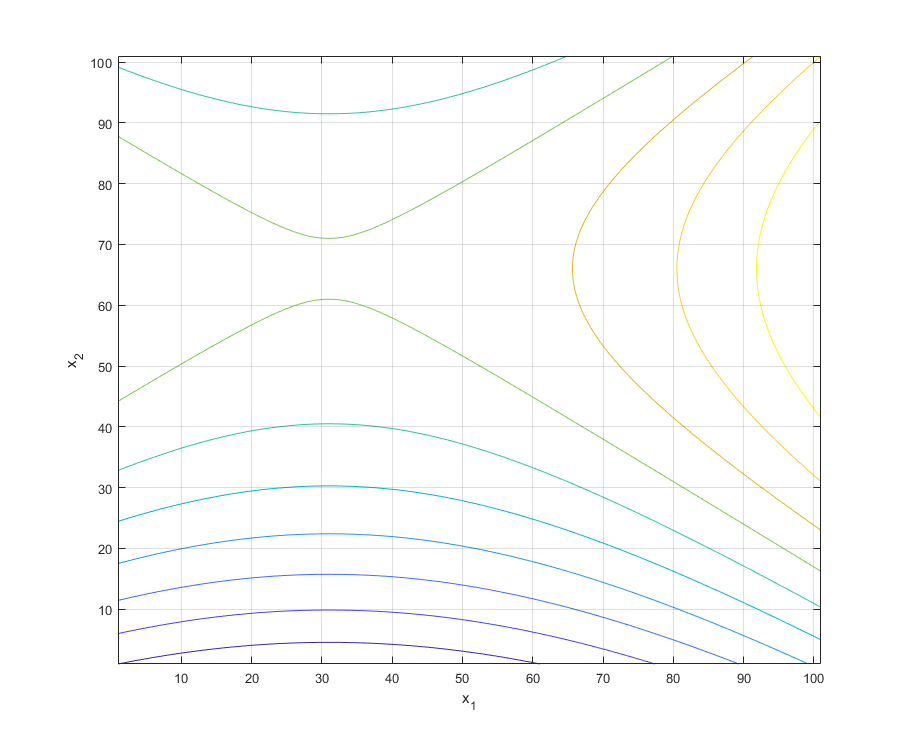
\includegraphics[width = .8\textwidth]{ContourLines.png}    
    \end{center}

    \end{enumerate}
\end{enumerate}

\begin{itemize}
    \item For $f: \mathbb{R}^2\rightarrow \mathbb{R}$ the \textbf{gradient} of $f$ is given by
    \[\nabla f(\mathbf{x})=\begin{bmatrix}\frac{\partial f}{\partial x_1}\\\frac{\partial f}{\partial x_2}\end{bmatrix},\]
    and the \textbf{Hessian} is the $2 \times 2$ matrix given by
    \[H = \nabla^2 f(\mathbf{x}) = \begin{bmatrix}\frac{\partial^2 f}{\partial x_1^2} & \frac{\partial^2 f}{\partial x_1 \partial x_2}\\\frac{\partial^2 f}{\partial x_2 \partial x_1} &\frac{\partial^2 f}{\partial x_2^2}\end{bmatrix}\]
    \textbf{Contour lines}, are found by studying the set of all \emph{level sets}, defined as
    \[\mathcal{L}_c(f) = \{(x_1,x_2) \mid f(x_1,x_2) = c\},\]
    where $c\in \mathbb{R}$ 
    
\end{itemize}
\end{document}
